\documentclass{beamer}
\usepackage[utf8]{inputenc}
\usepackage[T1]{fontenc}
\usepackage{amsmath}
\usepackage
[
    backend=biber,
    style=alphabetic,
    sortlocale=pl_PL,
    citestyle=alphabetic,
]{biblatex}
\usepackage{amssymb}
\usepackage{amsthm}
\usepackage{ebproof}
\usepackage{graphicx}
\usepackage{epstopdf}
\usepackage{inputenc}
\usepackage{MnSymbol}
\usepackage{mathtools}
\usepackage{geometry}
\usepackage{polski}
\usepackage{plain}
\usepackage{float}
\usepackage{epstopdf}
\usepackage{caption}
\usepackage{subcaption}
\usepackage{color}
\usepackage{url}
\usepackage{tikz-cd}
\usepackage{tikz}
\usetikzlibrary{matrix}
\usepackage{indentfirst}
\usepackage{multicol}
\usepackage{pdfpages}
\usepackage{import}
\usepackage{cases}
\usepackage{enumerate}
\usepackage{braket}
\usepackage{blindtext}
\usepackage{enumitem}
\usepackage[ampersand]{easylist}
\usepackage{mathbbol}

\DeclareSymbolFontAlphabet{\amsmathbb}{AMSb}%

\title{Kostka \(\lambda\)}
\usetheme{Warsaw}
%\usetheme{Madrid}

\begin{document}

\frame{
%  \frametitle{\(\lambda_{\rightarrow}\)}

  \begin{figure}[h]
    \centering
    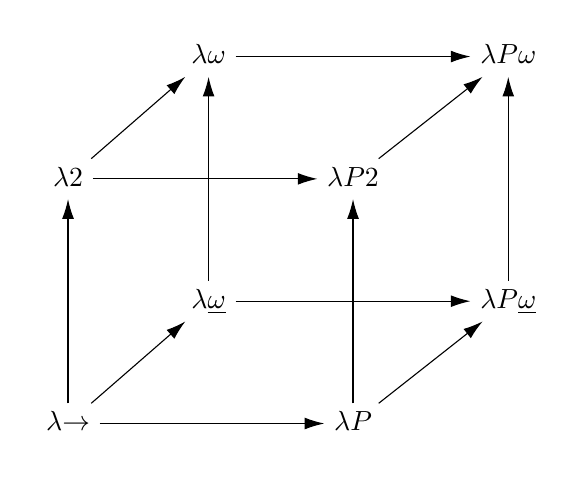
\begin{tikzpicture}[ampersand replacement=\&]
    \matrix (m) [matrix of math nodes,
    row sep=3em, column sep=3em,
    text height=1.5ex,
    text depth=0.25ex]{
                \& \lambda\omega             \&              \& \lambda P\omega             \\
    \lambda 2   \&                           \& \lambda P 2                                \\
                \& \lambda\underline{\omega} \&              \& \lambda P\underline{\omega} \\
    \lambda{\to}\&                           \& \lambda P  \\
    };
    \path[-{Latex[length=2.5mm, width=1.5mm]}]
    (m-1-2) edge (m-1-4)
    (m-2-1) edge (m-2-3)
            edge (m-1-2)
    (m-3-2) edge (m-1-2)
            edge (m-3-4)
    (m-4-1) edge (m-2-1)
            edge (m-3-2)
            edge (m-4-3)
    (m-3-4) edge (m-1-4)
    (m-2-3) edge (m-1-4)
    (m-4-3) edge (m-3-4)
            edge (m-2-3);
    \end{tikzpicture}
    \caption{Kostka \(\lambda\) H. Barendregta}
  \end{figure}
}

\frame{
  \frametitle{\(\lambda_{\rightarrow}\)}
  \begin{tabular}{l c c l}
  Typy: &
    \(\mathbb{T}\) & := &
      \(\mathbb{V}\)\\
  \vspace{0.5cm}
  & & | &\(\mathbb{T}\to\mathbb{T}\)\\
  Pseudotermy: &
    \(\mathbb{\Lambda_{T}}\) & := &
      \(V\)\\
  & & | &\(\mathbb{\Lambda_T \Lambda_T}\)\\
  & & | &\(\lambda V:\mathbb{T}.\,\mathbb{\Lambda_T}\)\\
  \end{tabular}\\
}

\frame {
  \frametitle{\(\lambda_{\rightarrow}\)}
  \begin{tabular}{l l}
  \vspace{0.5cm}
    Konteksty: & \(\Gamma = \{x_1 : A_1,\,\dots,\,x_n : A_n\}\)\\
    Redukcja:  & \((\lambda x:A.\,M)N\longrightarrow_{\beta} M[x:=N]\)
  \end{tabular}
}
\frame {
  \frametitle{\(\lambda_{\rightarrow}\)}
  Typizacja: \(\Gamma \vdash M : A\)\\

  \begin{center}
    \begin{tabular}{l c}  
    \vspace{0.5cm}
      (Var) &
      {\begin{prooftree}
        \Hypo{}
        \Infer1[]{\Gamma, x:A\vdash x:A}
      \end{prooftree}}\\
    \vspace{0.5cm}

      (App) &
      {\begin{prooftree}
        \Hypo{\Gamma \vdash M:A \to B} \Hypo{ \Gamma \vdash N:A}
        \Infer2[]{\Gamma \vdash (MN):B}
      \end{prooftree}}\\
      
    \vspace{0.5cm}
      (Abs) &
      {\begin{prooftree}
        \Hypo{ \Gamma, x:A \vdash M:B }
        \Infer1[]{\Gamma \vdash (\lambda\, x:A.\, M):A\to B}
      \end{prooftree}}\\
    \vspace{0.5cm}
    \end{tabular}
  \end{center}
}

\frame {
  \frametitle{\(\lambda T\)}
  \(0 : \mathbf{0}\)

  \(S : \mathbf{0} \to \mathbf {0}\)

  \(R_{\sigma} : \sigma \to (\sigma \to \mathbf{0} \to \sigma) \to \mathbf{0} \to \sigma\)
}
\frame{
  \frametitle{\(\lambda 2\) - termy zależne od typów}
  \begin{figure}[h]
    \centering
    \begin{tikzpicture}[ampersand replacement=\&]
    \matrix (m) [matrix of math nodes,
    row sep=3em, column sep=3em,
    text height=1.5ex,
    text depth=0.25ex]{
                \& \lambda\omega             \&              \& \lambda P\omega             \\
    \lambda 2   \&                           \& \lambda P 2                                \\
                \& \lambda\underline{\omega} \&              \& \lambda P\underline{\omega} \\
    \lambda{\to}\&                           \& \lambda P  \\
    };
    \path[-{Latex[length=2.5mm, width=1.5mm]}]
      (m-1-2) edge (m-1-4) [dotted]
    (m-2-1) edge (m-2-3)
            edge (m-1-2)
    (m-3-2) edge (m-1-2)
            edge (m-3-4)
      (m-4-1) edge [solid, thick] (m-2-1)
            edge (m-3-2)
            edge (m-4-3)
    (m-3-4) edge (m-1-4)
    (m-2-3) edge (m-1-4)
    (m-4-3) edge (m-3-4)
            edge (m-2-3);
    \end{tikzpicture}
  \end{figure}
}

\frame{
  \frametitle{\(\lambda 2\) - termy zależne od typów}
  \begin{tabular}{l c c l}
  Typy: &
    \(\mathbb{T}\) & := &
      \(\mathbb{V}\)\\
      & & | &\(\mathbb{T}\to\mathbb{T}\)\\
  \vspace{0.5cm}
      & & | &\(\forall \mathbb{V}.\,\mathbb{T}\)\\ 
  Pseudotermy: &
    \(\mathbb{\Lambda_{T}}\) & := &
      \(V\)\\
      & & | &\(\mathbb{\Lambda_T \Lambda_T}\)\\
      & & | &\(\lambda V:\mathbb{T}.\,\mathbb{\Lambda_T}\)\\
      & & | &\(\mathbb{\Lambda_T}\mathbb{T}\)\\
      & & | &\(\Lambda \mathbb{V.\, \Lambda_T}\)\\
  \end{tabular}\\
}
\frame{
  \frametitle{\(\lambda 2\) – termy zależne od typów}

  \begin{tabular}{l l}
  \vspace{0.5cm}
    Konteksty: & \(\Gamma = \{x_1 : A_1,\,\dots,\,x_n : A_n\}\)\\
    Redukcja:  & {$\!\begin{aligned}
      (\lambda a:A.\,M)N &\longrightarrow_{\beta} M[a:=N]\\
        (\Lambda \alpha.\, M) A &\longrightarrow_{\beta} M[\alpha:= A]
      \end{aligned}$}
  \end{tabular}
}
\frame {
  \frametitle{\(\lambda 2\) - termy zależne od typów}
  Typizacja: \(\Gamma \vdash M : A\)\\
  \begin{center}
  \begin{tabular}{r c c}

    \vspace{0.5cm}
    (Var) &
    {\begin{prooftree}
      \Hypo{}
      \Infer1[]{\Gamma, x:A\vdash x:A}
    \end{prooftree}} & \\
    \vspace{0.5cm}

    (App) &
    {\begin{prooftree}
      \Hypo{\Gamma \vdash M:A \to B} \Hypo{ \Gamma \vdash N:A}
      \Infer2[]{\Gamma \vdash (MN):B}
    \end{prooftree}} & \\
    \vspace{0.5cm}

    (Abs) &
    {\begin{prooftree}
      \Hypo{ \Gamma, a:A \vdash M:B }
      \Infer1[]{\Gamma \vdash (\lambda\, a:A.\, M):A\to B}
    \end{prooftree}} & \\
    \vspace{0.5cm}

    (\(\forall\)E) &
    {\begin{prooftree}
      \Hypo{ \Gamma \vdash M:(\forall \alpha.\,A)}
      \Infer1[]{\Gamma \vdash M B : A[\alpha:=B]}
    \end{prooftree}} &
    \(B \in \mathbb{T}\)  \\
    \vspace{0.5cm}

    (\(\forall\)I) &
    {\begin{prooftree}
      \Hypo{\Gamma \vdash M:A }
      \Infer1[]{\Gamma \vdash (\Lambda \alpha.\,M):(\forall \alpha.\,A)}
    \end{prooftree}} &
    \(\alpha\not\in \mathrm{FV}(\Gamma)\)  \\
  \end{tabular}
  \end{center}

}
\frame{
  \frametitle{\(\lambda \underline{\omega}\) - typy zależne od typów}
  \begin{figure}[h]
    \centering
    \begin{tikzpicture}[ampersand replacement=\&]
    \matrix (m) [matrix of math nodes,
    row sep=3em, column sep=3em,
    text height=1.5ex,
    text depth=0.25ex]{
                \& \lambda\omega             \&              \& \lambda P\omega             \\
    \lambda 2   \&                           \& \lambda P 2                                \\
                \& \lambda\underline{\omega} \&              \& \lambda P\underline{\omega} \\
    \lambda{\to}\&                           \& \lambda P  \\
    };
    \path[-{Latex[length=2.5mm, width=1.5mm]}]
      (m-1-2) edge (m-1-4) [dotted]
    (m-2-1) edge (m-2-3)
            edge (m-1-2)
    (m-3-2) edge (m-1-2)
            edge (m-3-4)
    (m-4-1) edge (m-2-1)
            edge [solid, thick] (m-3-2)
            edge (m-4-3)
    (m-3-4) edge (m-1-4)
    (m-2-3) edge (m-1-4)
    (m-4-3) edge (m-3-4)
            edge (m-2-3);
    \end{tikzpicture}
  \end{figure}
}

\frame{
  \frametitle{\(\lambda\underline{\omega}\) – typy zależne od typów}
  \begin{tabular}{l c c l}
  Pseudowyrażenia: &
    \(\mathcal{T}\) & := &
      \(V\)\\
    & & | &\(C\)\\
    & & | &\(\mathcal{T}\mathcal{T}\)\\
    & & | &\(\lambda V:\mathcal{T}.\,\mathcal{T}\)\\
    & & | &\(\mathcal{T}\to\mathcal{T}\)\\
  \end{tabular}\\
  \vspace{1cm}
  gdzie:\\ 
  \(V\) - przeliczalnie nieskończony zbiór zmiennych,\\
  \(C\) - zbiór stałych, w tym dwie szczególne nazywane \emph{sortami}: \(*,\,\Box\)
}
\frame{
  \frametitle{\(\lambda\underline{\omega}\) – typy zależne od typów}

\emph{Sądami} nazywamy wyrażenia \(\lambda\underline{\omega}\) postaci \(M:A\), gdzie \(M,\, A\in\mathcal{T}\)\\

\vspace{0.5cm}
\emph{Kontekstem} nazywamy skończony, liniowo uporzadkowany zbiór sądów. 
\\
\vspace{0.5cm}
\(<>\) oznacza kontekst pusty. Jeżeli \(\Gamma=<x_1:A_n,\,\dots, x_n:A_n>\), to wówczas \(\Gamma, y:B = <x_1:A_1, \,\dots, x_n:A_n, y:B>\).

}

\frame{
  \frametitle{\(\lambda\underline{\omega}\) – typy zależne od typów}
  Typizacja: \(\Gamma \vdash M : A\)\\
  \begin{center}
  \begin{tabular}{r c c }

    \vspace{0.2cm}
    (Ax) &
    {\begin{prooftree}
      \Hypo{}
      \Infer1[]{<>\vdash *:\Box}
    \end{prooftree}} & \\
    \vspace{0.2cm}

    (Start) &
    {\begin{prooftree}
      \Hypo{\Gamma \vdash A:s}
      \Infer1[]{\Gamma, x:A \vdash x:A}
    \end{prooftree}} & 
    \(x\not\in\Gamma\) \\
    \vspace{0.2cm}

    (Weak) &
    {\begin{prooftree}
      \Hypo{ \Gamma, A:B \vdash C:s }
      \Infer1[]{\Gamma, x:C \vdash A:B}
    \end{prooftree}} & 
    \(x\not\in\Gamma\)\\
    \vspace{0.2cm}

    (Type/Kind) &
    {\begin{prooftree}
      \Hypo{ \Gamma \vdash A:s} \Hypo{\Gamma \vdash B:s}
      \Infer2[]{\Gamma \vdash (A\to B):s }
    \end{prooftree}} & \\
    \vspace{0.2cm}

    (App) &
    {\begin{prooftree}
      \Hypo{\Gamma \vdash F:A\to B } \Hypo{\Gamma \vdash (A\to B) : s}
      \Infer2[]{\Gamma \vdash Fa:B}
    \end{prooftree}} & \\
    \vspace{0.2cm}

    (Abs) &
    {\begin{prooftree}
      \Hypo{\Gamma, x:A \vdash b:B } \Hypo{\Gamma \vdash (A\to B) : s}
      \Infer2[]{\Gamma \vdash (\lambda x:A.\,b):(A\to B)}
    \end{prooftree}} & \\
    \vspace{0.2cm}

    (Conv) &
    {\begin{prooftree}
      \Hypo{\Gamma \vdash A:B} \Hypo{\Gamma \vdash B':s } \Hypo{B =_{\beta} B'}
      \Infer3[]{\Gamma \vdash A:B'}
    \end{prooftree}} & \\

  \end{tabular}
  \end{center}
}

\frame{
  \frametitle{\(\lambda P\) - termy zależne od typów}
  \begin{figure}[h]
    \centering
    \begin{tikzpicture}[ampersand replacement=\&]
    \matrix (m) [matrix of math nodes,
    row sep=3em, column sep=3em,
    text height=1.5ex,
    text depth=0.25ex]{
                \& \lambda\omega             \&              \& \lambda P\omega             \\
    \lambda 2   \&                           \& \lambda P 2                                \\
                \& \lambda\underline{\omega} \&              \& \lambda P\underline{\omega} \\
    \lambda{\to}\&                           \& \lambda P  \\
    };
    \path[-{Latex[length=2.5mm, width=1.5mm]}]
      (m-1-2) edge (m-1-4) [dotted]
    (m-2-1) edge (m-2-3)
            edge (m-1-2)
    (m-3-2) edge (m-1-2)
            edge (m-3-4)
    (m-4-1) edge (m-2-1)
            edge (m-3-2)
            edge [solid, thick] (m-4-3)
    (m-3-4) edge (m-1-4)
    (m-2-3) edge (m-1-4)
    (m-4-3) edge (m-3-4)
            edge (m-2-3);
    \end{tikzpicture}
  \end{figure}
}


\frame{
  \frametitle{\(\lambda P\) – typy zależne od termów}

  \begin{tabular}{l c c l}
  Pseudowyrażenia: &
    \(\mathcal{T}\) & := &
      \(V\)\\
    & & | &\(C\)\\
    & & | &\(\mathcal{T}\mathcal{T}\)\\
    & & | &\(\lambda V:\mathcal{T}.\,\mathcal{T}\)\\
    & & | &\(\Pi V:\mathcal{T}.\,\mathcal{T}\)\\
  \end{tabular}\\
  \vspace{1cm}
  gdzie:\\ 
  \(V\) - przeliczalnie nieskończony zbiór zmiennych,\\
  \(C\) - zbiór stałych, w tym dwie szczególne nazywane \emph{sortami}: \(*,\,\Box\)


%  \begin{definition}
%    \begin{center}
%    \((A\to B) \equiv \Pi a : A.\,B\)
%    \end{center}
%  \end{definition}
}

\frame{
  \frametitle{\(\lambda P\) – typy zależne od typów}
  Typizacja: \(\Gamma \vdash M : A\)\\
  \begin{center}
  \begin{tabular}{r c c }

    \vspace{0.2cm}
    (Ax) &
    {\begin{prooftree}
      \Hypo{}
      \Infer1[]{<>\vdash *:\Box}
    \end{prooftree}} & \\
    \vspace{0.2cm}

    (Start) &
    {\begin{prooftree}
      \Hypo{\Gamma \vdash A:s}
      \Infer1[]{\Gamma, x:A \vdash x:A}
    \end{prooftree}} & 
    \(x\not\in\Gamma\) \\
    \vspace{0.2cm}

    (Weak) &
    {\begin{prooftree}
      \Hypo{ \Gamma, A:B \vdash C:s }
      \Infer1[]{\Gamma, x:C \vdash A:B}
    \end{prooftree}} & 
    \(x\not\in\Gamma\)\\
    \vspace{0.2cm}

    (Type/Kind) &
    {\begin{prooftree}
      \Hypo{ \Gamma \vdash A:*} \Hypo{\Gamma, x:A \vdash B:s}
      \Infer2[]{\Gamma \vdash (\Pi x:A.\, B):s }
    \end{prooftree}} & \\
    \vspace{0.2cm}

    (App) &
    {\begin{prooftree}
      \Hypo{\Gamma \vdash F:(\Pi x:A.\, B)} \Hypo{\Gamma \vdash a : A}
      \Infer2[]{\Gamma \vdash Fa:B[x:=a]}
    \end{prooftree}} & \\
    \vspace{0.2cm}

    (Abs) &
    {\begin{prooftree}
      \Hypo{\Gamma, x:A \vdash b:B } \Hypo{\Gamma \vdash (\Pi x:A.\, B) : s}
      \Infer2[]{\Gamma \vdash (\lambda x:A.\,b):(\Pi x:A.\, B)}
    \end{prooftree}} & \\
    \vspace{0.2cm}

    (Conv) &
    {\begin{prooftree}
      \Hypo{\Gamma \vdash A:B} \Hypo{\Gamma \vdash B':s } \Hypo{B =_{\beta} B'}
      \Infer3[]{\Gamma \vdash A:B'}
    \end{prooftree}} & \\

  \end{tabular}
  \end{center}
}

\frame{
  \frametitle{Kostka \(\lambda\)}
  \begin{figure}[h]
    \centering
    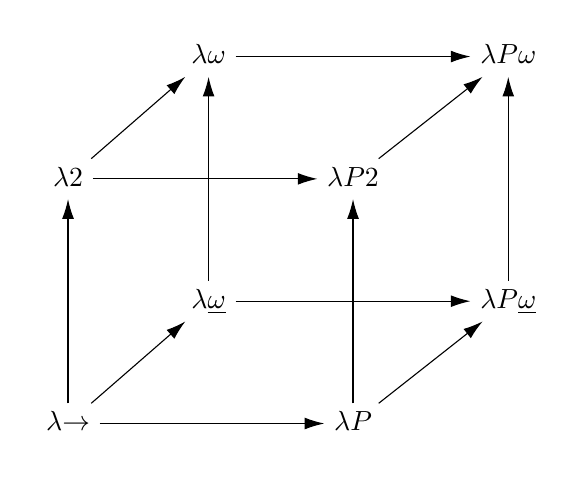
\begin{tikzpicture}[ampersand replacement=\&]
    \matrix (m) [matrix of math nodes,
    row sep=3em, column sep=3em,
    text height=1.5ex,
    text depth=0.25ex]{
                \& \lambda\omega             \&              \& \lambda P\omega             \\
    \lambda 2   \&                           \& \lambda P 2                                \\
                \& \lambda\underline{\omega} \&              \& \lambda P\underline{\omega} \\
    \lambda{\to}\&                           \& \lambda P  \\
    };
    \path[-{Latex[length=2.5mm, width=1.5mm]}]
    (m-1-2) edge (m-1-4)
    (m-2-1) edge (m-2-3)
            edge (m-1-2)
    (m-3-2) edge (m-1-2)
            edge (m-3-4)
    (m-4-1) edge (m-2-1)
            edge (m-3-2)
            edge (m-4-3)
    (m-3-4) edge (m-1-4)
    (m-2-3) edge (m-1-4)
    (m-4-3) edge (m-3-4)
            edge (m-2-3);
    \end{tikzpicture}
  \end{figure}
}
\frame{
  \frametitle{Kostka \(\lambda\)}
  \begin{tabular}{l c c l}
  Pseudowyrażenia: &
    \(\mathcal{T}\) & := &
      \(V\)\\
    & & | &\(C\)\\
    & & | &\(\mathcal{T}\mathcal{T}\)\\
    & & | &\(\lambda V:\mathcal{T}.\,\mathcal{T}\)\\
    & & | &\(\Pi V:\mathcal{T}.\,\mathcal{T}\)\\
  \end{tabular}\\
  \vspace{1cm}
  gdzie:\\ 
  \(V\) - przeliczalnie nieskończony zbiór zmiennych,\\
  \(C\) - zbiór stałych, w tym dwie szczególne nazywane \emph{sortami}: \(*,\,\Box\)

}

\frame{
  \frametitle{Kostka \(\lambda\)}
  \begin{tabular}{l l}
  \vspace{0.5cm}
    Redukcja:  & {$\!\begin{aligned}
      (\lambda x:A.\,B)C &\longrightarrow_{\beta} B[x:=C]
      \end{aligned}$}
  \end{tabular}
}

\frame{
  \frametitle{Kostka \(\lambda\)}
  W sądzie \(A:B\), gdzie \(A,\,B\in\mathcal{T}\), \(A\) nazywamy \emph{podmiotem}, zaś \(B\) – \emph{orzeczeniem}.\\

  \vspace{0.5cm}
\emph{Deklaracjami} nazywamy sekwenty sądy postaci \(x:A\), gdzie \(A\in\mathcal{T}\) i \(x\) jest zmienną.
}

\frame{
  \frametitle{Kostka \(\lambda\)}
  \emph{Psedokontekstem} nazywamy skończony, liniowo  uporządkowany zbiór deklaracji dla wzajemnie różnych podmiotów.
}

\frame{
  \frametitle{Kostka \(\lambda\)}
  Typizacja: \(\Gamma \vdash M : A\)\\

  Schematy reguł dzielimy na dwie grupy:

%  \begin{enumerate}
%      \item Reguły ogólne
%      \item Reguły wyróżniające
%  \end{enumerate}
}

\frame{
  \frametitle{Kostka \(\lambda\)}
a) Reguły ogólne
  \begin{center}
  \begin{tabular}{r c c }

    \vspace{0.2cm}
    (Ax) &
    {\begin{prooftree}
      \Hypo{}
      \Infer1[]{<>\vdash *:\Box}
    \end{prooftree}} & \\
    \vspace{0.2cm}

    (Start) &
    {\begin{prooftree}
      \Hypo{\Gamma \vdash A:s}
      \Infer1[]{\Gamma, x:A \vdash x:A}
    \end{prooftree}} & 
    \(x\not\in\Gamma\) \\
    \vspace{0.2cm}

    (Weak) &
    {\begin{prooftree}
      \Hypo{ \Gamma, A:B \vdash C:s }
      \Infer1[]{\Gamma, x:C \vdash A:B}
    \end{prooftree}} & 
    \(x\not\in\Gamma\)\\
    \vspace{0.2cm}

%    (Type/Kind) &
%    {\begin{prooftree}
%      \Hypo{ \Gamma \vdash A:*} \Hypo{\Gamma, x:A \vdash B:s}
%      \Infer2[]{\Gamma \vdash (\Pi x:A.\, B):s }
%    \end{prooftree}} & \\
%    \vspace{0.2cm}

    (App) &
    {\begin{prooftree}
      \Hypo{\Gamma \vdash F:(\Pi x:A.\, B)} \Hypo{\Gamma \vdash a : A}
      \Infer2[]{\Gamma \vdash Fa:B[x:=a]}
    \end{prooftree}} & \\
    \vspace{0.2cm}

    (Abs) &
    {\begin{prooftree}
      \Hypo{\Gamma, x:A \vdash b:B } \Hypo{\Gamma \vdash (\Pi x:A.\, B) : s}
      \Infer2[]{\Gamma \vdash (\lambda x:A.\,b):(\Pi x:A.\, B)}
    \end{prooftree}} & \\
    \vspace{0.2cm}

    (Conv) &
    {\begin{prooftree}
      \Hypo{\Gamma \vdash A:B} \Hypo{\Gamma \vdash B':s } \Hypo{B =_{\beta} B'}
      \Infer3[]{\Gamma \vdash A:B'}
    \end{prooftree}} & \\

  \end{tabular}
  \end{center}
}

\frame{
  \frametitle{Kostka \(\lambda\)}
b) Reguły wyróżniające
  \begin{center}
  \begin{tabular}{r c c }
    (\((s_1, s_2)\)-reguła ) &
    {\begin{prooftree}
      \Hypo{ \Gamma \vdash A:s_1} \Hypo{\Gamma, x:A \vdash B:s_2}
      \Infer2[]{\Gamma \vdash (\Pi x:A.\, B):s_2 }
    \end{prooftree}} & \\

  \end{tabular}
  \end{center}
}

\frame{
  \begin{center}
  \begin{tabular}{r | l | c c c c}
    0 & \(\lambda_{\to}\)                 & \((*,\,*)\) \\
    1 & \(\lambda 2\)                     & \((*,\,*)\) & \((\Box,\,*)\) \\
    2 & \(\lambda P\)                     & \((*,\,*)\) & & \((*,\,\Box)\) \\
    1+2 & \(\lambda P2\)                  & \((*,\,*)\) & \((\Box,\,*)\) & \((*,\,\Box)\) \\
    3 & \(\lambda \underline{\omega}\)    & \((*,\,*)\) & & & \((\Box,\,\Box)\)\\ 
    1+3 & \(\lambda \omega\)              & \((*,\,*)\) & \((\Box,\,*)\) & & \((\Box,\,\Box)\)\\ 
    2+3 & \(\lambda P\underline{\omega}\) & \((*,\,*)\) & & \((*,\,\Box)\) & \((\Box,\,\Box)\) \\
    1+2+3 & \(\lambda C\)                 & \((*,\,*)\) & \((\Box,\,*)\) & \((*,\,\Box)\) & \((\Box,\,\Box)\) \\
  \end{tabular}
  \end{center}
}
\end{document}
